\documentclass[12pt]{letter}\usepackage[letterpaper,margin=0.65in]{geometry}\usepackage{textcomp}\usepackage{graphicx}\usepackage[rflt]{floatflt}\pagenumbering{gobble}\begin{document}\begin{floatingfigure}{0.15\textwidth}\raisebox{0pt}[0pt][0pt]{\raisebox{-2.5cm}{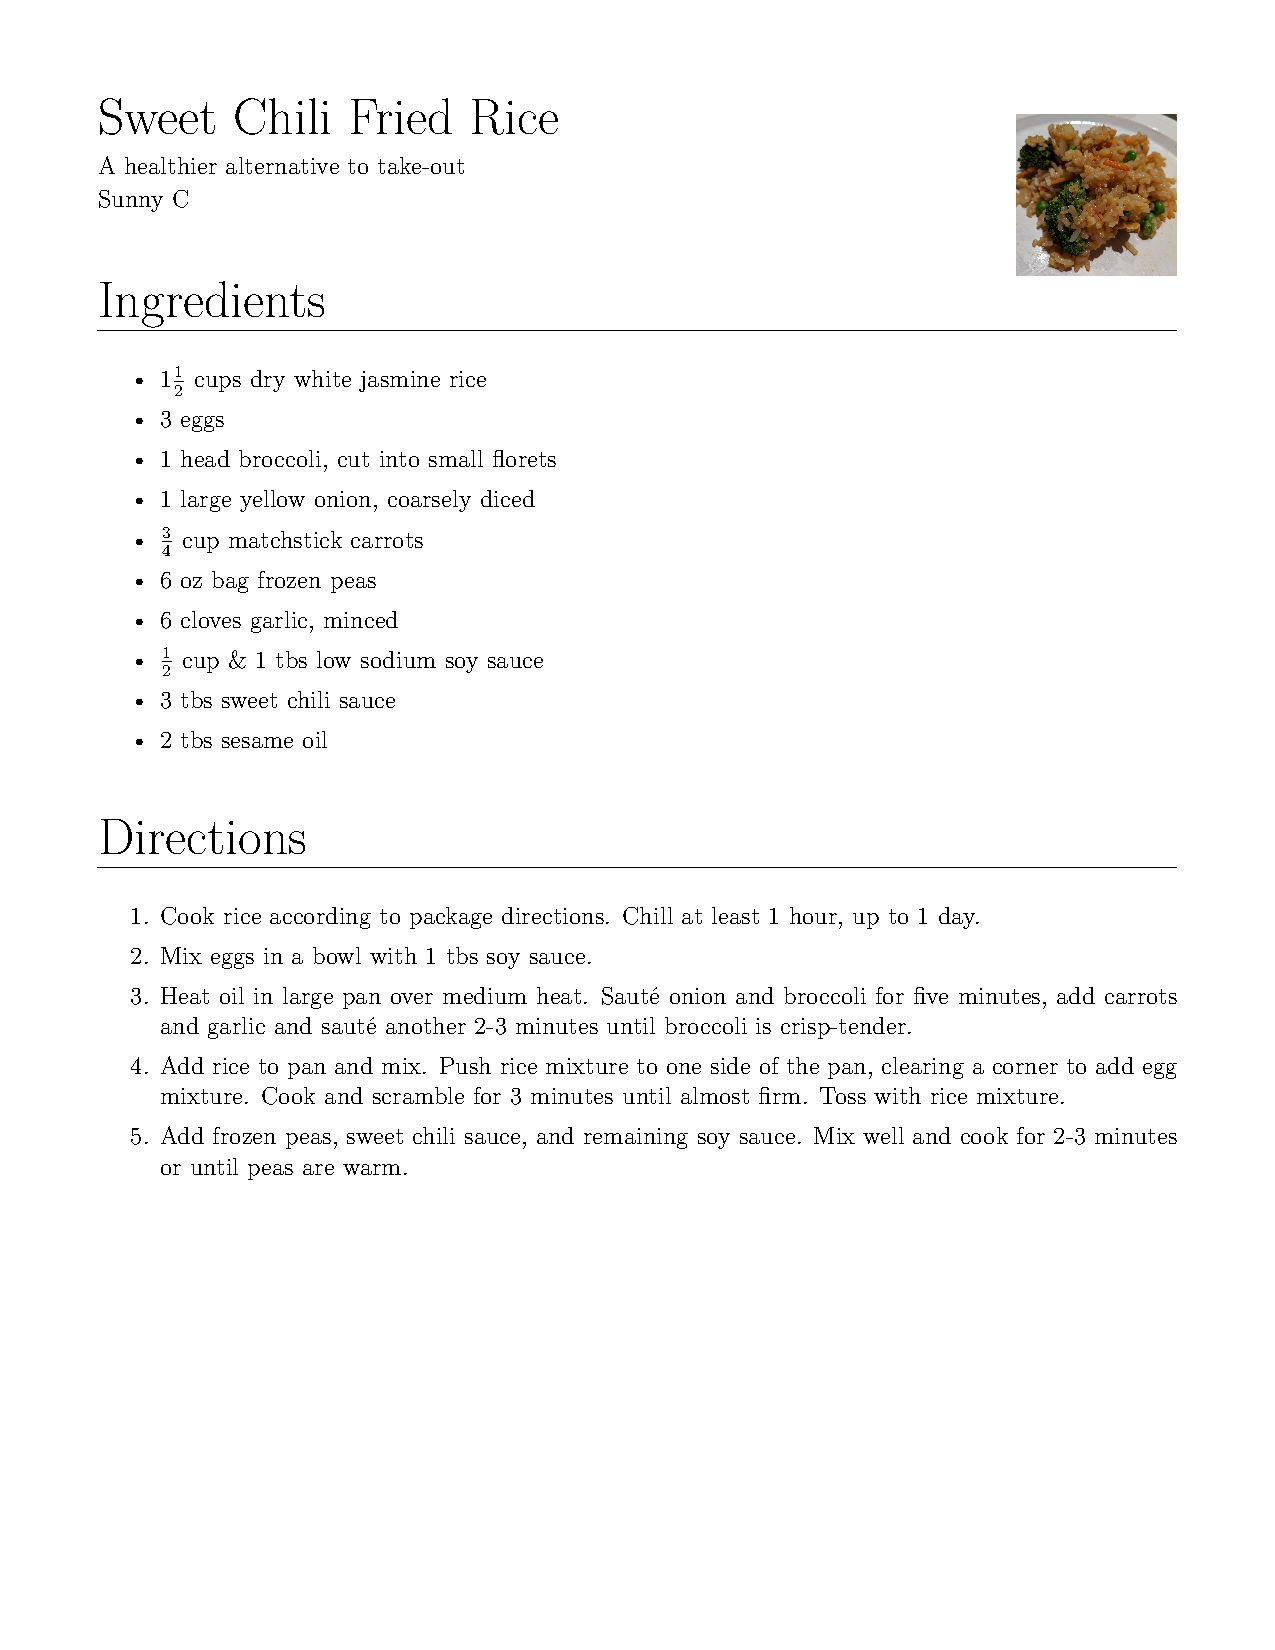
\includegraphics[width=0.15\textwidth]{sweet-chili-fried-rice}}}\end{floatingfigure}\begin{huge}Sweet Chili Fried Rice\end{huge}\newline\vspace{-2.5mm}\newline\renewcommand{\arraystretch}{1.1}\begin{tabular*}{\textwidth}{@{\extracolsep{\fill}}lr}A healthier alternative to take-out\\Sunny C\end{tabular*}\newline\vspace{10mm}\newline\begin{huge}Ingredients\end{huge}\\\rule[2.8mm]{\textwidth}{.1pt}\vspace{-3mm}\begin{itemize}\item 1$\frac{1}{2}$ cups dry white jasmine rice\item 3 eggs\item 1 head broccoli, cut into small florets\item 1 large yellow onion, coarsely diced\item $\frac{3}{4}$ cup matchstick carrots\item 6 oz bag frozen peas\item 6 cloves garlic, minced\item $\frac{1}{2}$ cup \& 1 tbs low sodium soy sauce\item 3 tbs sweet chili sauce\item 2 tbs sesame oil\end{itemize}\vspace{7mm}\begin{huge}Directions\end{huge}\\\rule[2.8mm]{\textwidth}{.1pt}\vspace{-3mm}\begin{enumerate}\item Cook rice according to package directions. Chill at least 1 hour, up to 1 day.\item Mix eggs in a bowl with 1 tbs soy sauce.\item Heat oil in large pan over medium heat. Sauté onion and broccoli for five minutes, add carrots and garlic and sauté another 2-3 minutes until broccoli is crisp-tender.\item Add rice to pan and mix. Push rice mixture to one side of the pan, clearing a corner to add egg mixture. Cook and scramble for 3 minutes until almost firm. Toss with rice mixture.\item Add frozen peas, sweet chili sauce, and remaining soy sauce. Mix well and cook for 2-3 minutes or until peas are warm.\end{enumerate}\end{document}